% ES definition: scan tokens until target language detected
\documentclass[tikz,border=5pt]{standalone}
\usetikzlibrary{arrows.meta}
\begin{document}
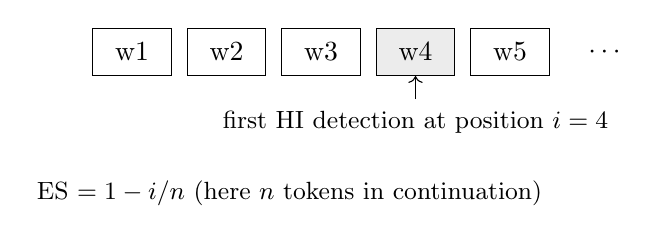
\begin{tikzpicture}[
  node distance=6mm,
  box/.style={draw, minimum width=10mm, minimum height=6mm, align=center},
  line/.style={->}
]
\node[box] (t1) at (0,0) {w1};
\node[box] (t2) at (12mm,0) {w2};
\node[box] (t3) at (24mm,0) {w3};
\node[box, fill=gray!15] (t4) at (36mm,0) {w4};
\node[box] (t5) at (48mm,0) {w5};
\node (dots) at (60mm,0) {$\cdots$};

\node at (36mm,-9mm) {\small first HI detection at position $i=4$};
\draw[->] (36mm,-6mm) -- (t4.south);

\node at (20mm,-18mm) {\small ES $= 1 - i/n$ (here $n$ tokens in continuation)};
\end{tikzpicture}
\end{document}

